\section{Topología del Plano Complejo}
Los conceptos de {\it Compacidad} y {\it Conexidad} se asumen como conocidos. 

A lo largo del libro se utilizará la siguiente notación de topología de conjuntos: 
Si $A$ es un subconjunto de un espacio topológico $X$, su cerradura (adherencia) 
se denota por $\closureSet{A}$ y su interior por $\interiorSet{A}$. Su frontera 
$\closureSet{A} \setminus \interiorSet{A}$ se denota por $\partial A$. Si $X$ es además 
un espacio métrico con distancia $d$, la distancia de un punto $x \in X$ a un 
subconjunto $A\subset X$ se denota y se define por $d(x, A) = \displaystyle \inf_{a \in A} d(x,a)$.

\subsection{Conjuntos abiertos de C}

\begin{theo}
Cualquier subconjunto $\Omega$ abierto y no vacío de $\mathbb{C}$ se puede 
escribir como la unión exhaustiva de una sucesión creciente $(K_n)_{n \geq 1}$ 
de subconjuntos compactos, es decir,
$$
\Omega = \bigcup_{n=1}^{\infty} K_n, \, \text{ donde }\, K_n \subset \interiorSet{K}_{n+1}, \, \forall n \geq 1.
$$
\end{theo}
\begin{dem}
{\bf La idea de la demostración es construir una sucesión creciente
 de conjuntos cerrados y acotados, contenidos en $\Omega$, y que 
 eventualmente cubran todo $\Omega$. Para consideraremos dos conjuntos,
 un compacto que crezca arbitrariamente, y otro }

    Para cada $n\geq 1$, definamos 
    \begin{equation*}
        K_n = \left \{  z\in \mathbb{C} \tq |z| \leq n  \right \} 
        \bigcap 
        \left \{  z\in \mathbb{C} \tq d(z, \Omega^{c})\geq 1/n \right \}.
    \end{equation*}

    Los $K_n$ forman una sucesión creciente de conjuntos cerrados y acotados (pues para cada $n$ se cumple que 
    $\{  z\in \mathbb{C} \tq |z| \leq n  \} \subset \{  z\in \mathbb{C} \tq |z| \leq n+1  \}$ 
    y también $\{  z\in \mathbb{C} \tq d(z, \Omega^{c})\geq 1/n \} \subset \{  z\in \mathbb{C} \tq d(z, \Omega^{c})\geq 1/(n+1) \}$), 
    luego por el Teorema de Heine-Borel estos son compactos. 
    Además cada $K_n$ está contenido en $\Omega$ 
    (pues $\left\{  z\in \mathbb{C} \tq d(z, \Omega^{c})\geq 1/n \right\} \subset \Omega$), 
    entonces $\displaystyle \cup_{n}K_n \subset \Omega$. Por otro lado, para cualquier $z\in \Omega$,  
    tenemos que $d(z,\Omega^{c}) > 0$, por lo tanto existe $n_0\geq 1$  tal que $d(z,\Omega^{c})\geq 1/n_0$. 
    También, existe un natural $n_1\geq 1$ tal que $\abs{z} \leq n_1$, luego tomando $N=\max\{n_0, n_1\}$ 
    se sigue que $d(z,\Omega^{c})\geq 1/N$ y  $\abs{z} \leq N$, esto es, $z\in K_N \subset \cup_n Kn$. 
    Por lo tanto, $\displaystyle \cup_{n}K_n = \Omega$.  

    Ahora probemos que $K_n \subset \interiorSet{K}_{n+1}, \, \forall n \geq 1$. Para esto observe 
    que para cada $n$, los conjuntos 
    $\Omega_n = \left \{ z\in \mathbb{C} \tq |z| < n  \right \} \cap \left \{  z\in \mathbb{C} \tq d(z, \Omega^{c})> 1/n \right \}$, 
    son abiertos y además $K_{n-1} \subset \Omega_n \subset K_n$. Ya que el interior de un conjunto es 
    el conjunto abierto más grande contenido él, se sigue que para cada $n$, $K_n \subset \Omega \subset \interiorSet{K}_{n+1}$.
    
    Por último, que la unión es \textit{exhaustiva} significa que no solamente cualquier punto de $\Omega$ 
    pertenece a alguno de los $K_n$, sino más aún que cualquier subconjunto compacto $K \subset \Omega$ 
    también está contenido en alguno de los $K_n$. Consideremos un compacto $K$ tal que $K\subset \Omega$. 
    De que $K_n \subset \interiorSet{K}_{n+1}$, se sigue que $\Omega = \cup_n \interiorSet{K}_{n+1}$, 
    luego tenemos una cubierta abierta para $K$. De aquí el lector puede terminar el argumento usando 
    la compacidad de $K$.
\end{dem}
%Ejemplo de cita: Como se menciona en \cite{hardy2008numbers}, los números primos son fundamentales.

\subsection{Conjuntos Conexos de C}

Dados un $a\in \C$  y $r>0$, definimos y denotamos al disco abierto centrado en $a$ y de radio $r$ por:
\[ D(a,r) = \{ z\in \C\; : \; |z - a| < r \}. \]

\begin{figure}[H]
    \centering
    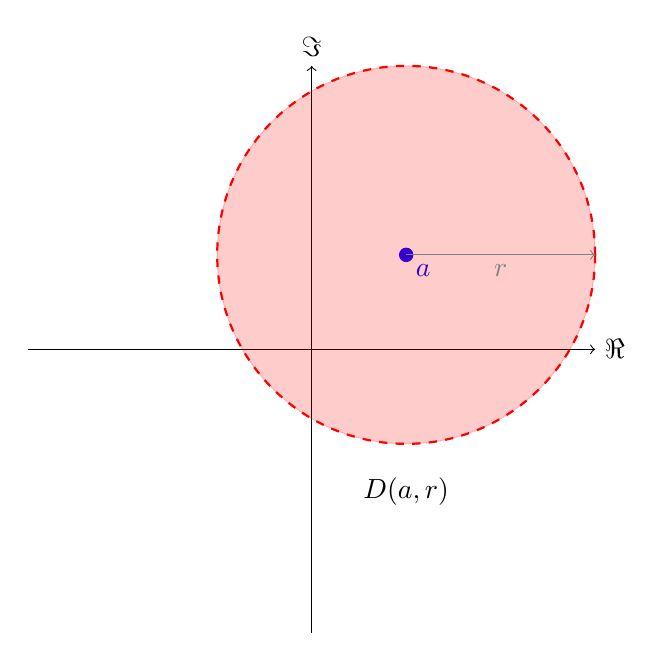
\begin{tikzpicture}[scale=1.2]
    
      % Ejes
      \draw[->] (-3,0) -- (3,0) node[right] {\(\Re\)};
      \draw[->] (0,-3) -- (0,3) node[above] {\(\Im\)};
    
      % Punto 'a'
      \filldraw[blue] (1,1) circle (2pt) node[below right] {\(a\)};
      
      % Disco abierto centrado en 'a' con radio 'r'
      \draw[red, thick, dashed] (1,1) circle (2);
      \filldraw[red, opacity=0.2] (1,1) circle (2);
      
      % Etiqueta del radio
      \draw[gray, ->] (1,1) -- (3,1) node[midway, below] {\(r\)};
      
      % Texto D(a, r)
      \node at (1,-1.5) {\(D(a, r)\)};
    
    \end{tikzpicture}
    \caption{Disco abierto \( D(a, r) \subset \mathbb{C} \), centrado en el punto \( a \) con radio \( r \).}
    \label{fig:disco_abierto}
\end{figure}
    
\begin{theo}
    Sea $\Omega$ un subconjunto abierto de $\C$. Entonces las componentes conexas de $\Omega$ son abiertas, y la
    colección de estas componentes conexas es a lo más numerable.
\end{theo}
\begin{dem}
    Veamos primero que las componentes conexas son conjuntos abiertos. 
    Sea $C$ una componente conexa arbitraria de $\Omega$, y sea $a \in C$ un elemento arbitrario. \\
    P.D. Existe $r>0$ tal que $D(a, r) \subset C$.\\
    En efecto, como $a \in C \subset \Om$, y $\Om$ es abierto se sigue que existe $r>0$ tal que $D(a,r) \subset \Om$.
    Por otro lado, $D(a,r)$ es conexo, y $D(a,r)\cap C \neq \emptyset$, luego $D(a,r)\cup C$ es conexo. Como $C$ es 
    una componente conexa por definición es maximalmente conexo, con lo que $D(a,r) \subset C$ (de lo contrario 
    tendriamos $C \subsetneq D(a,r)\cup C$).

    Para ver que la colección de componentes conexas de $\Om$ es a lo más numerable basta con checar que podemos elegir
    un punto con coordenadas racionales en cada componente. Esto se garantiza gracias a que cada componente es abierta, 
    y que $\Q\times \Q$ es denso en $\C$.
\end{dem}

Por lo que hemos visto hasta el momento podemos intuir que los conjuntos abiertos, los conjuntos compactos y los 
conjuntos conexos serán de particular importancia, y que en lo sucesivo debemos prestar mucha atención en cómo 
sacarles provecho. El siguiente resultado nos señala que también los complementos de los conjuntos compactos son 
de gran interés, así pues también debemos mantenerlos bajo nuestro radar, y aprender a aprovechar sus bondades.

\begin{theo}
    Sea $K$ un compacto de $\C$ y $\Om = \C \setminus K$. Entonces
    \begin{enumerate}
        \item De las componentes conexas del abierto $\Om$ solo una es no acotada, $C_{\infty}$.
        \item Si $C$ es una componente conexa de $\Om$, entonces $\partial C \subset K$.
    \end{enumerate}
\end{theo}
\begin{dem}
    Veamos primero que de las componentes conexas de $\Om = \C \setminus K$ solo hay una que es no acotada. En efecto,
    como $K$ es compacto, es cerrado y acotado, luego existe $R > 0$ tal que $K \subset D(O, R) = \vcentcolon D$.
    Observemos que $D^c$ es conexo y no acotado. Por otro lado, $R \in \Om$ y $R\in D^c$, entonces $D^c$ está contenido
    en la componente conexa de $\Om$ que contiene a $R$, $C_R$. Observando que todas las otras posibles componentes conexas de
    $\Om$ se encuentran dentro de $D$, se sigue que $C_R$ es la única que es no acotada, la cuál se denotará por $C_{\infty}$.

    Por último, consideremos una componente conexa arbitraria, $C$, de $\Om$. Por el teorema anterior se sigue que $C$ es abierto
    en $\C$ y cerrado en $\Om$, pues $C=\closureSet{C}\cap \Om$ (por ser $C$ un subconjunto de maximalmente conexo $\Om$). Luego, 
    $$
    \partial C = \closureSet{C}\setminus C = \closureSet{C}\setminus (\closureSet{C}\cap \Om) =
    \closureSet{C}\cap (\closureSet{C}\cap \Om)^c= \closureSet{C}\cap(\closureSet{C}^c \cup \Om^c) =
    \closureSet{C} \cap K \subset K.
    $$
\end{dem}
\begin{figure}[H]
    \centering
    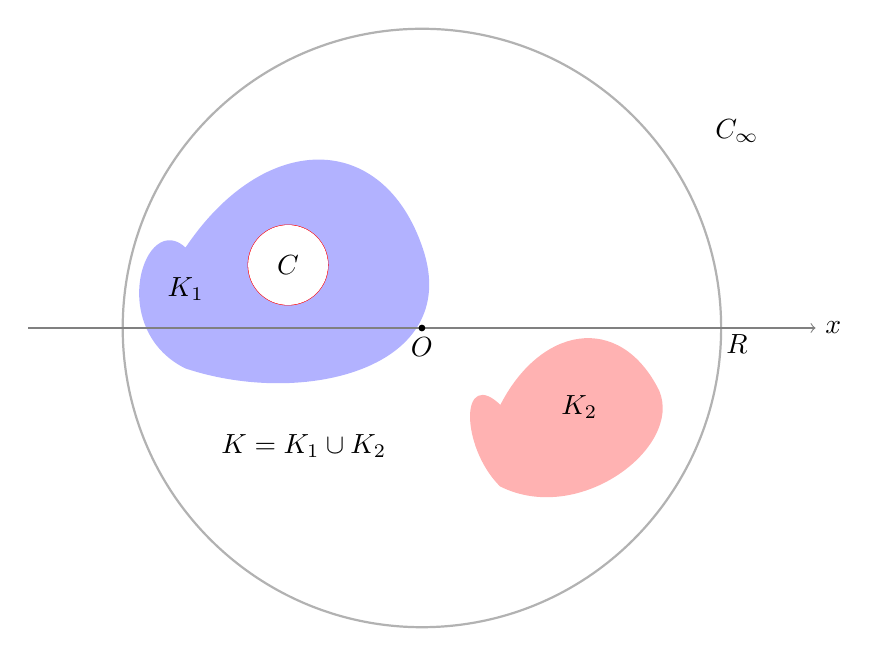
\begin{tikzpicture}[scale=1.0]
      
      % K1: conjunto compacto con agujero
      \begin{scope}
        % Contorno exterior suave       
        \filldraw[blue!30, thick, smooth cycle]
          (-3,1) .. controls (-2,2.5) and (-0.5,2.5) .. (0,1)
                 .. controls (0.5,-0.5) and (-1.5,-1) .. (-3,-0.5)
                 .. controls (-4,0) and (-3.5,1.5) .. (-3,1);
        
                 
        % Agujero interior
        \draw[red, thick] (-1.7,0.8) circle (0.5);
        \filldraw[white] (-1.7,0.8) circle (0.5);
        %\filldraw[white, smooth cycle]
        %  (1,0) .. controls (1.5,0.5) and (2,0.5) .. (2,0)
        %        .. controls (2,-0.5) and (1.5,-0.5) .. (1,-0.2)
        %        .. controls (0.8,0) and (0.9,0.1) .. (1,0);
      \end{scope}
      % Etiqueta C
      \node at (-1.7,0.8) {\(C\)};
      % Etiqueta K1
      \node at (-3,0.5) {\(K_1\)};
      
      % K2: conjunto compacto separado, forma irregular
      \filldraw[red!30, thick, smooth cycle]
        (1,-1) .. controls (1.5,0) and (2.5,0.2) .. (3,-0.8)
              .. controls (3.3,-1.5) and (2,-2.5) .. (1,-2)
              .. controls (0.5,-1.5) and (0.5,-0.5) .. (1,-1);
      
      % Etiqueta K2
      \node at (2,-1) {\(K_2\)};

      % Etiqueta K
      \node at (-1.5,-1.5) {\(K = K_1 \cup K_2\)};
      % Disco encerrando K1 y K2:
      \draw[black!30, thick] (0,0) circle (3.8);
      % Etiqueta radio R
      \node at (4,-.2) {\(R\)};

      % Etiqueta C_infty
      \node at (4,2.5) {\(C_{\infty}\)};
      % Ejes
      \draw[->, gray] (-5,0) -- (5,0) node[right, black] {\(x\)};
      %\draw[->] (0,-3) -- (0,3) node[above] {\(\Im\)};
      % Origen
      \filldraw[black] (0,0) circle(1pt) node[below] {\(O\)} ;
      % Etiqueta Origen : O
      %\node at (0,-0.2) {\(O\)};
    \end{tikzpicture}
    \caption{ El conjunto \( K = K_1 \cup K_2 \) es un compacto de \( \C\).}
    \label{fig:compactos_disjuntos}
  \end{figure}

  %%%%%%%%%%%%%%%%%%%%%%%%%%%%%%%%%%%%%%%%%%%%%%% Fin de la section %%%%%%%%%%%%%%%%%%%5

 